% ABLS - term-long paper

\documentclass{sig-alternate}

\usepackage{url}
\usepackage{color}
\usepackage{enumerate}
\usepackage{balance}
\usepackage{verbatim}
\usepackage{enumitem}
\usepackage[table]{xcolor}
\usepackage{multicol,multirow}
\usepackage{subfig}
\usepackage{dcolumn}
\usepackage{palatino}
\usepackage{bbm}
\usepackage{url}
\usepackage{verbatim}
\usepackage{algorithm}
\usepackage[noend]{algorithmic}
\usepackage{fancybox, fancyvrb}
\usepackage{listings}
\usepackage{amsmath}
\usepackage{array}

\newenvironment{definition}[1][Definition]{\begin{trivlist}
\item[\hskip \labelsep {\bfseries #1}]}{\end{trivlist}}

\permission{}
\CopyrightYear{2012}
%\crdata{0-00000-00-0/00/00}
\begin{document}

\title{ABLS: Enabling Attribute-Based Logging and Automated Auditing in the Cloud}
\numberofauthors{1}
\author{
\alignauthor{
Christopher A. Wood \\
Department of Computer Science \\
{\tt caw4567@rit.edu}
}}
\date{\today}
\maketitle
\begin{abstract}
User-based non-repudiation is an increasingly important property of cloud-based applications. It provides irrefutable 
evidence that ties system behavior to specific users, thus enabling strict enforcement of organizational security policies. 
System logs are typically used as the basis for this property. Thus, the effectiveness of system audits based on log files 
reduces to the problem of maintaining the integrity and confidentiality of log files without sacrificing the usefulness
of the data in these log files. In an ideal setting, automated audits would be possible on encrypted log data that defines
audit trails. Furthermore, since useful log messages may contain sensitive information, access control for log 
data should be implemented so as to restrict access to only those parties that need to view it (i.e. generating users,
colleagues of generating users, auditors, system administrators, etc). ABAC has been a common technique used to
satisfy this requirement. %with the expense of role explosion. 

In this paper we address all of the aforementioned issues with ABLS, an attribute-based logging system designed
to support automates audits of encrypted audit trails (log data) based on user-defined security policies. Access to
sensitive log information is enforced using ciphertext-policy attribute-based encryption (CP-ABE) with a minimal number
of log-related roles, and thus a small number of attributes, to avoid the problem of increasing encryption computational
complexity with attribute explosion. We present the preliminary design of ABLS and discuss how audit trails are 
constructed, automated audit tasks are defined and specified, and how the system may be used in practical applications.
\end{abstract}

\section{Introduction}
User-based non-repudiation is a system security property that provides indisputable evidence linking
specific actions to individual users (or entities) that trigger such actions. Cryptographically speaking, 
non-repudiation requires that the integrity and 
origin of all data should be provable. In essence, this enables system audits to be conducted that can
identify data misuse, and thus, potential security policy violations, by comparing the contextual information 
of system events (e.g. source user, time of the event, etc) with all entities authorized to invoke such events. 
Therefore, treating non-repudiation as a required system quality attribute in the architecture is likely to 
become a common trend in the commercial, government, and even more specifically, the health-care domain.

System audits typically use log files to determine the ``who, what, when, and how'' of events that took 
place during the system's lifetime. In order to provide accurate information for non-repudiation purposes,
it is often necessary to place some amount user-sensitive data in these log files that can be used
to trace data back to its origin. As such, logs of events generated by a client that is being served must
maintain data confidentiality and integrity should the system be compromised. Historical approaches
to the problem of log security are based on tamper-resistant hardware and maintaining continuous 
secure communication channels between a log aggregator and end user \cite{Schneier1999-Secure}. 
However, such solutions are not applicable in the context of cloud-based applications. 

Recent approaches have relied on combinations of encryption and signature techniques \cite{Ma2008-FssAgg}. 
Symmetric-key and public-key encryption (and verification) of log entries are very common confidentiality techniques 
proposed in the literature. Unfortunately, these schemes are becoming less useful in cloud-based applications.
There is a need for robust access control mechanisms that enable dynamic user addition and revocation
with minimal overhead. In other words, continuously re-encrypting a subset of the log database should be avoided. 
Both symmetric- and public-key cryptosystems suffer in that access policies must be tied directly to keys used for
encryption and decryption. If the access policy for a set of log messages needs to be changed, then both the keys used to
encrypt and decrypt such log entries will need to be regenerated and distributed, and the entries must also
be re-encrypted. Both of these tasks can be very expensive. 

In addition, symmetric-key cryptosystems require keys to be shared among users who need access to the 
same set of logs. This requires a secure and comprehensive key management and distribution scheme and
supporting policy. In a similar vein, public-key cryptosystems (e.g. RSA and ElGamal) suffer 
from the extra data transfer and storage requirements for large cryptographic keys and certificates. There 
may be insufficient resources to maintain a public-key infrastructure (PKI) for managing keys and digital 
certificates for all users. 

In terms of log file integrity, aggregate signature schemes that support forward secrecy through the use of 
symmetric- and public-key cryptosystems are also becoming outdated \cite{Yavuz2009-BAF}. 
Symmetric-key schemes may promote high computational efficiency for signature generation, but they 
do not directly support public verifiability for administrators and auditors. This means that robust key 
distribution schemes or the introduction of a trusted third party (TTP) are needed to ensure that all 
required parties can verify the necessary log data. Such schemes also 
suffer from relatively high storage requirements and communication overhead. Public-key 
schemes have similar issues, as the increased key size leads to even larger storage 
requirements and less computational efficiency. Also, public-key schemes introduce the need
for a trusted certificate authority to grant certificates for all parties that sign log information. % TODO: find a citation for this...
One time-tested technique for supporting log file integrity is the use of authenticated 
hash-chains \cite{Schneier1999-Secure}, which will be the focus of this paper.

Collectively, we see that a balance between encryption and signature generation and verification performance is
needed to support the unique scalability and resource usage requirements for cloud-based applications.
Furthermore, the selected cryptographic primitives to encrypt, sign, and verify data must not exacerbate the
problem of dynamically changing access control policies and user privileges. Role-based Access Control (RBAC),
which first gained popularity in the mid 1990s \cite{Sandhu1996-RBAC} \cite{David1992-RBAC} and was later 
proposed as a standard for the National Institute of Standards and Technology in 2001\cite{Ferraiolo2001-RBAC}, 
is an increasingly popular access control policy that enables users to be associated with roles that change
less frequently. In the context of maintaining the confidentiality of log messages generated by many users,
RBAC surpasses traditional mandatory and discretionary access control (MAC and DAC) 
\cite{Abrams1990-AccessControl}.

More recently, attribute-based access control (ABAC) \cite{TODOTODO} has been developed to 
provide fine-grained access control to sensitive data. It is common practice to specify user roles as attributes
in this access control scheme, thus enabling the benefits of RBAC with fine-grained access control.
Attribute-based encryption (ABE) \cite{Goyal2006-ABAC}, a new cryptographic scheme that uses 
user attributes (or roles, in this context) to maintain the confidentiality of user-sensitive data, has an appealing application
to logging systems maintained in the cloud and is capable of satisfying the aforementioned confidentiality 
requirements. 

In this paper we address all of the aforementioned issues with ABLS, an attribute-based logging system designed
to support automates audits of encrypted audit trails (log data) based on user-defined security policies. Access to
sensitive log information is enforced using ciphertext-policy attribute-based encryption (CP-ABE) with a minimal number
of log-related roles, and thus a small number of attributes, to avoid the problem of increasing encryption computational
complexity with attribute explosion. We present the preliminary design of ABLS and discuss how audit trails are 
constructed, automated audit tasks are defined and specified, and how the system may be used in practical applications.

The paper is organized in a top-down fashion, starting with the structure of log data and corresponding ability
to define automated audit tasks. Using this foundation, we then introduce the relational data model used to persist
log information, followed by the cryptographic access control mechanisms used to maintain the confidentiality
of log data and audit trails. Finally, we conclude with a practical use case for ABLS in the context of healthcare 
organizations.

\section{Structured Log Data and Automated Audits}
A major motivating factor for our log data structure comes from realistic security policies. In this context, we make
the assumption that a security policy can be stated as a set of \emph{negative} requirements. For example, one 
such requirement might be that a doctor is not allowed to change their patient's address. In order to conduct an 
automated audit for violations of this policy, we first translate this semantically-rich requirement into a language
whose structure can be easily mapped to a relational data model. This enables us to leverage the power of 
structured query languages (i.e. SQL) to search for policy violations.

One solution for parsing security policy requirements into relational data is to define a grammar for producing 
requirement strings from a set of non-terminals that correspond to relations. Using the NIST RBAC model of
access control as motivation (TODO: CITE), we specify this set of non-terminals and relations to be the set identifiers 
$USER$, $OBS$, $OPS$, and $AFFECTEDUSERS$. These finite sets are minimal enough to allow the specification
of most security policies, thus making it suitable for our needs. 

LAudit, a simple context-free grammar that is built on these relations, is shown below.

%{\setlength\tabcolsep{4pt}
%\begin{tabular}{>{$}l<{$}>{$}r<{$}>{$}l<{$}}
%  \text{LAudit} &\Coloneqq & \text{USER OPS}\\
%  &| & \text{USER OPS OBS} \\
%  &| & \text{USER OPS OBS USER} \\
%\end{tabular}}

\vspace{.35cm} 
In this context, USER, OPS, and OBS are all finite sets composed of the users, operations, and objects of a
system, as specified by the NIST RBAC model \cite{Sandhu2000-nist-rbac}. While simple, this language effectively
captures the ``who'' and ``what'' of log events. ABLS is capable of appending a timestamp to every that it receives,
which rounds off the log event with ``when'' information. 

ABLS clients must submit log messages according to a pre-defined schema that captures
all of the information in LAudit. The JSON schema used for constructing log messages is shown below.

\begin{lstlisting}
[
    {
        user : int,
        session : int,
        action : int (or String),
        object : int (or String),
        affectedUsers : [int]
    }
]
\end{lstlisting}

In order to capture this information in a relational model to enable efficient queries, a new Event table was added
to the database schema. There is a one-to-one correspondence between Event 
and Log records, and the security of such Event
and Log information is maintained using the same hash chain construction techniques as in the preliminary design.
However, for simplicity, the notion of hash chain epochs was removed.
Also, Action, Object, and AffectedUserGroup tables were added to the database schema to store relevant information
about log events as they are received from the log proxy. A high-level depiction of this new relational model is shown
in Figure \ref{fig:design2}.

\begin{figure}[ht!]
\begin{center}
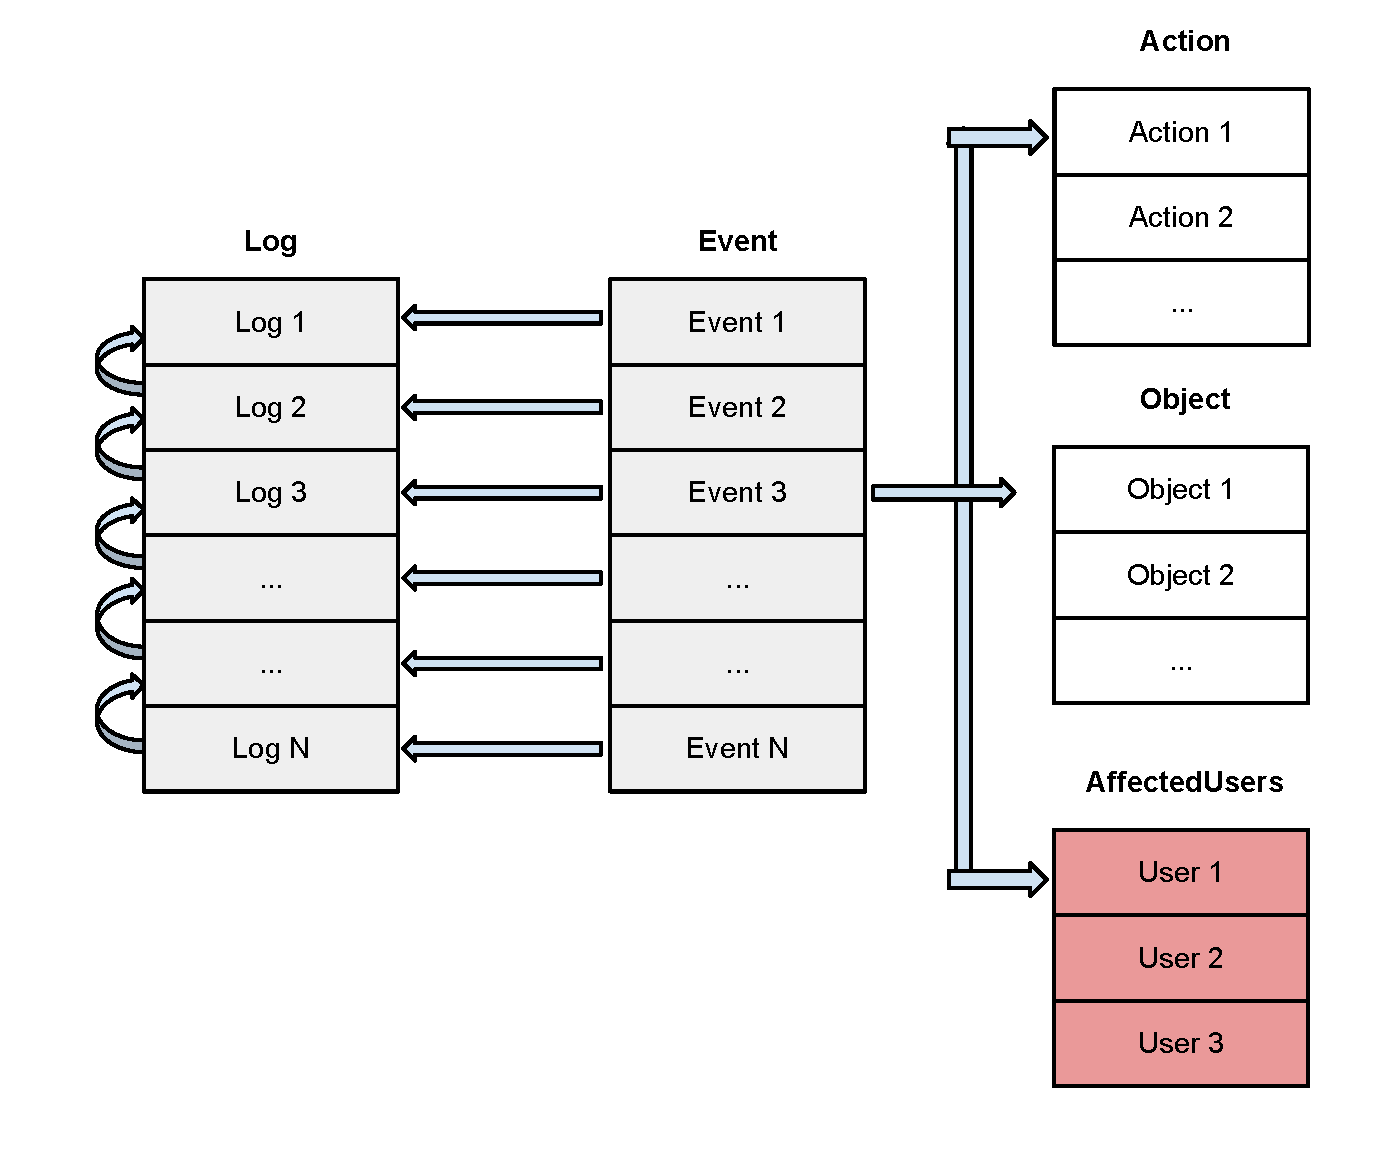
\includegraphics[width=3in]{images/relational_design_v2.pdf}
\caption{A high-level depiction of the new relational data model that supports automated audit tasks.}
\label{fig:design2}
\end{center}
\end{figure}

In this model, all Action and Object records are stored in plaintext. These tables store elements of a finite set, and
encrypting them would not deter a determined attacker. However, all information about affected users is encrypted 
(masked) using the same technique discussed in Section \ref{sec:databaseDesign}. As such, an attacker can infer
information about what types of objects were operated upon, but they cannot determine the specifics of these actions
or the users who performed them without compromising the ABLS master key $M_k$. We feel as though this strikes
a good balance between robust audit specification, reasonable measures of audit and log efficiency, and overall 
log security. 

Audit tasks enforce audit rules using a blacklist approach. Audit rules are specified using the aforementioned 
log message schema and then assigned to audit tasks that periodically run to see if the rules are being properly enforced.
For example, an audit rule might be configured as follows:


%define a grammar for specifying 
%If we consider the set of security policy requirements similar to the aforementioned example as a set of sentences
%accepted by a context-free language $L$, where the alphabet $\Sigma$ of $L$ is a set of finite users, actions, 
%objects, and other attributes (i.e. timestamps), 

%LAudit, a simple context-free grammar that is capable of producing such security policies, enables us to parse such 

%Parsing the semantics of such 
%a security policy 

%the details of such
%a policy snippet requires the log data to uniquely identify the doctor as a user generating an action, ``change'' as an
%action performed on an ``address'' object, and a patient as an affected user. It is natural to parse the semantics of
%this security policy 

%express such semantics
%using a formal language that captures users, objects, actions, and other important attributes that are general enough
%to allow the specification of any security policy.

%LAudit, a language for specifying audit log data, was created to fulfill this exact role. 


\section{Cryptography Preliminaries}
Ciphertext Policy Attribute-Based Encryption (CP-ABE) is a new encryption scheme that supports complex
access policies that specify which secret keys can be used for decryption. In CP-ABE, secret keys are analogous
to sets of attributes, and access policies are defined using a tree-like access structure of logical AND and OR
gates, where each leaf in the tree is an attribute \cite{Bethencourt2007-CPABE}. Implementations of 
CP-ABE schemes are usually based on the construction of a bilinear mapping between two elliptic curve 
groups \cite{Bethencourt2007-CPABE} \cite{Junod2010-ABE}. We define both of these terms in the following sections.

\subsection{Mathematical Foundations}
\begin{definition}
Let $\mathbb{F}_p$ be a finite field where $p > 3$ is a prime, and $a, b \in \mathbb{F}_p$ such that
\begin{align*}
4a^3 + 27b^2 \not= 0 \mod p \in \mathbb{F}_p
\end{align*}

An \emph{ellptic curve} $E[\mathbb{F}_p]$ is the set of solutions $(x, y)$ to the equation
\begin{align*}
y^2 = x^3 + ax + b \mod p \in \mathbb{F}_p[x],
\end{align*}
together with the point at infinite $0$.
\end{definition}

\begin{definition}
Let $G_1$ and $G_2$ be cyclic groups of prime order $p$ and $g$ a generator of $G_1$. We say that $e$ is a \emph{bilinear map} defined as $e : G_1 \times G_2$, where $|G_1| = |G_2| = p$. This bilinear map satisfies the following properties:
\begin{itemize}
	\item Bilinearity: For all $u, v \in G_0$ and $a, b \in \mathbb{Z}_p$, we have $e(u^a, v^b) = e(u,v)^{ab}$
	\item Non-degeneracy: $e(g, g,) \not= 1$
	\item Computability: Both $G_1$ and $G_2$ are efficiently computable
\end{itemize}
\end{definition}

\subsection{Ciphertext Policy Attribute-Based Encryption}
In the original construction of the CP-ABE scheme, Bethencourt et al. \cite{Bethencourt2007-CPABE} defined five different procedures 
used in the cryptosystem: \emph{Setup}, \emph{Encrypt}, \emph{KeyGeneration}, \emph{Derypt}, and 
\emph{Delegate}. We define each of these procedures as follows:
\begin{itemize}
	\item \textbf{Setup} - This procedure takes the implicit security parameter as input and outputs the public and master keys $PK$ and $MK$.
	\item \textbf{Encrypt}(\textbf{PK}, M, $\mathbb{A}$) - This procedure will encrypt $M$, a plaintext message, to produce a ciphertext $CT$ such that only a user that possesses a set of attributes that satisfies the access structure $\mathbb{A}$ will be able to decrypt the message. The encryption process embeds $\mathbb{A}$ into the ciphertext.
	\item \textbf{KeyGeneration}(\textbf{MK}, $\mathbb{S}$) - This procedure generates a private key $SK$ using the master key $MK$ and set of attributes $S$ that describe the private key. 
	\item \textbf{Decrypt}(\textbf{PK}, \textbf{CT}, \textbf{SK}) - This procedure decrypts the ciphertext $CT$ using the provided secret key $SK$ to return the original message $M$. Decryption is only successful if the set $S$ of attributes, which is associated with the key $SK$, satisfies the access policy embedded within the ciphertext (which is part of the access structure $\mathbb{A}$).
	\item \textbf{Delegate}(\textbf{SK}, \~{S}) - This procedure outputs a secret key \~{$SK$} for the set of attributes \~{$S$}, where \~{$S$} $\subset S$, the set of attributes associated with the secret key \textbf{SK}.
\end{itemize}

\section{Log Access Policies}
%%%% TODO: start proofreading here...
One of the motivating parts of this project was to explore the usefulness of CP-ABE schemes
for secure logging. The ability to embed robust access policies within the encrypted
ciphertext made this an appealing solution. The CP-ABE scheme also provides us with the ability to
enforce dynamic access to certain log entries using our policy engine (described in the next section),
prevent insider attacks by tying access to user attributes rather than user keys. Furthermore,
we avoid the need for a full-blown public or private key distribution scheme by encapsulating the secret
key generation process for encryption within the logging system. Key distribution is only needed when
decrypting log messages. We begin our discussion with a description of the access policies generated
by our policy engine, which is used to grant temporal access to certain log entries.

\subsection{Access Policy Definitions}
The policy engine in our logging scheme is motivated by the need to provide forward and backward security
for log entries (i.e. dynamic temporal access) with very fine grained role descriptions. In 
fact, user identities are the basis for access policies. This allows us to control explicit access to log entries based on individual
identities, in addition to the abstract notion of user roles. For example, if a user 
U1 and their colleagues U2, U3, and U4 should be the only ones to view log entries associated with a specific event E1, then the access 
policy for such log entries should be based on the identity of U1 and an attribute that describes
colleagues of U1. Such an access policy might be defined as follows.
\begin{align*}
\text{(User ID)} \lor \text{(Colleague of User)} \lor \text{(System Administrator)}
\end{align*}
With this rule, U1 will always be able to access the data (which is a fact that should never change), but 
colleagues must request access through the policy engine. Upon receiving a request, the policy engine would
check the colleagues of U1 at the current time against the requesting user, and if the requesting user
belongs to the set of colleagues of U1 they are granted the temporary colleague of U1 attribute to decrypt the data. 

%\subsection{Event-Specific Policies}
%TODO: how we tie events to policies
%Policy(event, source) = build based on source and the source rules for this event 
%users have a set of events associated with them (all events are enumerated), and then rules for each event

Our logging scheme makes the assumption that events, and the access policies for all data associated
with such events, are well defined. With this
assumption, we can represent the behavior of the policy engine by the system users and their associated
data, events, and policy rules for specific events. In this way, policy rules are coupled to events in that 
policies for access are generated based on the type of event that occurred and the user who is requesting 
access to such information. Policy rules can be thought of as functions similar to the one described by 
{\tt RuleE1} and {\tt RuleE2} (Algorithms \ref{alg:ruleE1} and \ref{alg:ruleE2}, respectively).
In this example, we see that the rule for event E1 
takes an {\tt EventInformation} structure, which contains
all of the information generated for an event. A prospective definition for an {\tt EventInformation} structure
is shown below.
\begin{lstlisting}
struct 
{
    User SourceUser;
    int EventId;
} 
EventInformation;
\end{lstlisting} 

The information contained within this structure is specific 
to the implementation of the system. For our purposes, we only require the source user from which the
event was generated, as well as the event identifier. The policy engine would then query the user
database to determine the secret identity of the source user and embed this in the resulting attribute
list. Optionally, depending on the implementation of {\tt RuleE1}, the policy engine would append additional
attributes to the list in disjunctive normal form. The simplicity of these policy implementations 
makes changing them an effortless task should the organization's security policy change.

\begin{algorithm}[t] %[htb]
\caption{{\tt RuleE1} policy implementation} \label{alg:ruleE1}
\begin{algorithmic}[1]
\REQUIRE{An {\tt EventInformation} object instance $e$.}
\ENSURE{The access policy for the event corresponding to the information in $e$}
\STATE{attributeId $\leftarrow$ database.queryUserId(e.SourceUser)}
\STATE{Return ('attributeID' OR 'Colleague of attributeID' OR 'System Administrator')}
\end{algorithmic}
\end{algorithm}

\begin{algorithm}[t] %[htb]
\caption{{\tt RuleE2} policy implementation} \label{alg:ruleE2}
\begin{algorithmic}[1]
\REQUIRE{An {\tt EventInformation} object instance $e$.}
\ENSURE{The access policy for the event corresponding to the information in $e$}
\STATE{attributeId $\leftarrow$ database.queryUserId(e.SourceUser)}
\STATE{Return ('attributeID' OR 'System Administrator')}
\end{algorithmic}
\end{algorithm}

\subsection{Key Generation and Management}
By default, the secret keys used for decryption are never cached in the system's local memory. Since it is
expected that log entries will be read much less frequently than they will be written, such keys are generated
on demand by querying the appropriate database. Furthermore, the key generation process can be done in two ways. 
For policy rules that limit the access to only the generating user, only a single query to the attribute database
is required to establish the user's secret key and then decrypt the data for all log entries corresponding to that rule. With this key
the user may decrypt these entries offline without the need to query the policy engine for the appropriate access rights.

Conversely, for access policy rules that embed conditions for colleagues or other users 
related to the source user, the policy engine must first query the
user database to ensure the requesting user meets the relationship criteria set in place by the policy. Then,
if this is successful, the policy engine will grant the appropriate secret key to the requesting user. The tradeoff
is that, while an online TTP is needed for such colleagues to access the log entry contents, it is significantly easier
for the system administrators to manage who has access to specific log entries aside from the original source user.
Simply modifying the user's relationships in the system database is sufficient to revoke access from certain colleagues.

In order to maintain the security of the system at runtime, it is necessary to cycle the master and public keys
associated with the encryption scheme. Our current system does not support this feature, but there are two
ways that it could be implemented. The first way is to persist the old master and 
public keys to a safe location that could be called during auditing and verification if needed. The second way is 
to re-encrypt the entire log database with the new master and public key. Unfortunately, this would not only require the system to be 
brought offline during the update (in order to avoid synchronization issues with live traffic), but it would also
mean that the new master and public key serve as a single point of failure for the entire database if compromised. 
Therefore, future releases of this system plan to implement the first approach to manage keys. It would be
best to determine the key cycle lifetime based on empirical data associated with the growth of the log database.
Intuitively, in order to maintain auditing and verification efficiency, the cycle frequency should be defined as 
a monotonically increasing function that is proportional to the growth of the database. 

\section{Use Case: Electronic Health Record Systems}
TODO

\begin{comment}
\begin{table}
\centering
\caption{Feelings about Issues}
\begin{tabular}{|l|r|l|} \hline
Flavor&Percentage&Comments\\ \hline
Issue 1 &  10\% & Loved it a lot\\ \hline
Issue 2 &  20\% & Disliked it immensely\\ \hline
Issue 3 &  30\% & Didn't care one bit\\ \hline
Issue 4 &  40\% & Duh?\\ \hline
\end{tabular}
\end{table}

\begin{figure}[htb]
\label{sample graphic}
\begin{center}
\includegraphics[width=1.5in]{fly.jpg}
\caption{A sample black \& white graphic (JPG).}
\end{center}
\end{figure}
\end{comment}

\bibliographystyle{abbrv}
\bibliography{../abls}
% You must have a proper ".bib" file
%  and remember to run:
% latex bibtex latex latex
% to resolve all references
\balance
\end{document}
